%%%%%%%%%%%%%%%%%%%%%%%%%%%%%%%%%%%%%%%%%%%%%%%%%%%%%%%%%%%%%%%%%%%%%%%%%%%%%%%%
\section{Databases And Capture Methods}\label{ch:bg_db_capture}
%%%%%%%%%%%%%%%%%%%%%%%%%%%%%%%%%%%%%%%%%%%%%%%%%%%%%%%%%%%%%%%%%%%%%%%%%%%%%%%%
In contrast to generic shape recovery, facial shape recovery implies a strong
assumption that the input image contains a face. This prior knowledge, that the
image contains a face, enables the use of training data to improve the
quality of the reconstruction. However, collection of this training data, which
may take the form of either direct 3D information (meshes, range images) or
functions of the facial surface (normals, parametric reflectance data) must
use accurate shape recovery methods in order to be useful. Therefore, the
collection of accurate facial shape for the purposes of providing approximate
ground truth data is a research topic in its own right. In this section, we
begin by discussing the existing 3D facial databases and the manner of their
collection. Following this, we discuss the details of the 3D recovery algorithms
and focus on works intended specifically for facial surface recovery.
%%%%%%%%%%%%%%%%%%%%%%%%%%%%%%%%%%%%%%%%
% CANDIDE 3d wireframe model
% MPI     7 views, 200 laser scanned heads, 5 full 3D, Cyberware, static, neutral
% ND-D    953 scans, Minolta Vivid 900 3D scanner, 656 subjects, neutral, static
% ND-2006 13,450 images containing 6 different types of expressions, 888 distinct people
%         Static, Minolta Vivid 910 range scanner
% 3D-TEC 212 individuals (106 twins),  Minolta VIVID 910 3D scanner, 1 neutral, 1 smiling, static
% CASIA 3D 4624 scans of 123 persons, Minolta Vivid 910, various poses, emotions, static
% B3D(AC)^2 scanned using \cite{weise2007fast}, 14 subjects, 1109 sequences, dynamic 25 FPS, reading
% BIWI Head Pose  15K images of 20 people, various head poses, missing frames, kinect
% UOY Face Database 97 people, multi-pose, neutral, smile and frown
% GavabDB 61 individuals, 427 images, multi pose, static, 3 expressions
% FRAV3D 106 subjects,  MINOLTA VIVID-700, multi-pose, static
% Basel 200 scans, neutral, ABW-3D structured light scanner
% BJUT-3D, cyberware
% EURECOM Kinect, 52 people * 18 image, multi poses, expressions, static
% XM2VTS stereo, 25 subjects, neutral,
% Texas 3DFRD 1149 pairs of facial color and range images of 105 adult human subjects,
%             stereo imaging system manufactured by 3Q Technologies, neutral, frontal
% ZJU-3DFED  40 subjects, total 360, expressions, InSpeck 3D MEGA Capturor DF
% 3D_RMA structured light, 120 people, 6 shots, multi-pose
% Beckmann cyberware, 400-500, single shot
% UMB-DB Minolta Vivid 900 laser scanner
\begin{table}
\centering
\resizebox{\textwidth}{!}{%
\begin{tabular}{@{}cccccccc@{}}
\toprule
\multicolumn{3}{c}{DB}                                                              & \# Subjects & \# Outputs  & Expressions  & Poses        & Type   \\ \midrule
CANDIDE v1                  &\cite{Rydfalk:1987tg}          & 1987                  & 1           & 1           & $\checkmark$ & ---          & MO     \\ \midrule
MPI                         &\cite{Troje:1996ep}            & 1996                  & 200         & 200         &              &              & M      \\ \midrule
CANDIDE v2                  &\cite{Ahlberg:1998uk}          & \multirow{2}{*}{1998} & 1           & 1           & $\checkmark$ & ---          & MO     \\
3D\_RMA                     &\cite{beumier2001face}         &                       & 120         & 720         &              & $\checkmark$ & D      \\ \midrule
USF                         &\cite{RefWorks:96}             & \multirow{3}{*}{1999} & 200         & 200         &              & ---          & MO     \\
XM2VTSdb                    &\cite{messer1999xm2vtsdb}      &                       & 295         & 2360        &              &              & M      \\
YaleB                       &\cite{RefWorks:314}            &                       & 10          & 5760        & $\checkmark$ &              & PS     \\ \midrule
CASIA 3D                    &\cite{casia3d}                 & \multirow{2}{*}{2003} & 123         & 1845        & $\checkmark$ &              & D      \\
FSU                         &\cite{hesher2003novel}         &                       & 37          & 222         & $\checkmark$ &              & D      \\ \midrule
GavabDB                     &\cite{moreno2004gavabdb}       & 2004                  & 61          & 720         & $\checkmark$ & $\checkmark$ & D      \\ \midrule
FRGC v2                     &\cite{phillips2005overview}    & 2005                  & 466         & 4007        & $\checkmark$ &              & D      \\ \midrule
BU3D-FE                     &\cite{Yin:2006cc}              & \multirow{4}{*}{2006} & 100         & 2500        & $\checkmark$ &              & M      \\
ND-2006                     &\cite{faltemier2007using}      &                       & 888         & 13450       & $\checkmark$ &              & D      \\
FRAV3D                      &\cite{conde2006multimodal}     &                       & 106         & 1696        & $\checkmark$ &              & M      \\
ZJU-3DFED                   &\cite{wang2006exploring}       &                       & 40          & 360         & $\checkmark$ &              & M      \\ \midrule
Beckmann                    &\cite{hu2007building}          & 2007                  & $\sim$400   &~?           & $\checkmark$ &              & M      \\ \midrule
Bosphorus                   &\cite{Savran:2008gg}           & \multirow{3}{*}{2008} & 105         & 4652        & $\checkmark$ &              & M      \\
UoY                         &\cite{heseltine2008three}      &                       & 350         & 5250        & $\checkmark$ & $\checkmark$ & M      \\
BU4D-FE                     &\cite{yin2008high}             &                       & 101         & Many        & $\checkmark$ & $\checkmark$ & 4D M   \\ \midrule
Basel                       &\cite{paysan20093d}            & \multirow{2}{*}{2009} & 200         & 200         &              & ---          & MO     \\
BJUT-3D                     &\cite{baocai2009bjut}          &                       & 500         & 500         &              &              & M      \\ \midrule
B3D (AC)\textsuperscript{2} &\cite{fanelli20103}            & \multirow{2}{*}{2010} & 14          & Many        & $\checkmark$ &              & 4D D/M \\
Texas 3DFRD                 &\cite{gupta2010anthropometric} &                       & 118         & 1149        &              &              & M      \\ \midrule
3D-TEC                      &\cite{vijayan2011twins}        & \multirow{4}{*}{2011} & 212         & 212         & $\checkmark$ &              & M      \\
BIWI Head Pose              &\cite{fanelli2013random}       &                       & 20          & $\sim$15000 &              & $\checkmark$ & D      \\
UMB-DB                      &\cite{colombo2011umb}          &                       & 143         & 1473        & $\checkmark$ &              & M      \\
Florence 3D                 &\cite{bagdanov2011florence}    &                       & 53          & 212         &              & $\checkmark$ & M      \\ \midrule
ICT-3DRFE                   &\cite{stratou2012exploring}    & \multirow{2}{*}{2012} & 23          & 345         & $\checkmark$ &              & PS     \\
Superfaces                  &\cite{berretti2012superfaces}  &                       & 20          &~?           &              & $\checkmark$ & M/D    \\ \midrule                               
Photoface                   &\cite{RefWorks:293}            & 2013                  & 261         & 1839        & $\checkmark$ &              & PS/M   \\ \midrule
FaceWarehouse               &\cite{Cao:2014gy}              & \multirow{3}{*}{2014} & 150         & 3000        & $\checkmark$ & ---          & MO/D   \\
BP4D-Spontaneous            &\cite{Zhang:2014id}            &                       & 41          & Many        & $\checkmark$ & $\checkmark$ & 4D M   \\
EURECOM                     &\cite{min2014kinectfacedb}     &                       & 52          & 936         & $\checkmark$ & $\checkmark$ & D      \\ \midrule
SURREY                      &\cite{Huber:F5Dca9zy}          & 2016                  & 169         & 169         &              & ---          & MO     \\ \bottomrule
\end{tabular}%
}
\caption{A timeline of existing 3D facial databases including depth data, mesh
         data, models and Photometric Stereo images. PS denotes Photometric
         Stereo images, MO is a statistical model, M is a 3D mesh, 
         D is depth/range data and 4D implies a 3D video.}
\label{tbl:timeline_db}
\end{table}
%%%%%%%%%%%%%%%%%%%%%%%%%%%%%%%%%%%%%%%%
%%%%%%%%%%%%%%%%%%%%%%%%%%%%%%%%%%%%%%%%%%%%%%%%%%%%%%%%%%%%%%%%%%%%%%%%%%%%%%%%
\subsection{Databases}\label{subsec:bg_databases}
%%%%%%%%%%%%%%%%%%%%%%%%%%%%%%%%%%%%%%%%%%%%%%%%%%%%%%%%%%%%%%%%%%%%%%%%%%%%%%%%
The collection of 3D facial databases has a rich history
that spans over many decades. \cref{tbl:timeline_db} provides a
timeline outlining these 3D facial databases and the composition of the 
data that they provide.
It is particularly interesting to note that, despite the fact that one of the
first 3D facial models was released in 1987 (CANDIDE~\cite{Rydfalk:1987tg}), the
majority of existing databases were produced in the last decade. The quality
of these facial models has also increased substantially, which is demonstrated
in \cref{fig:db_examples}. 

The CANDIDE~\cite{Rydfalk:1987tg,Ahlberg:1998uk} models were parametrizable
wireframe models that contained a low number of vertices (75--95) and were
designed to be controlled according to pre-defined Action Units. The CANDIDE
model was not captured from real data and thus had limited uses for modelling
identity. Early attempts at recording facial databases focused on the use
of laser scanning technology~\cite{cyberware,minolta} or structured light. For
example, the early work of \citet{beumier2001face} used an internally developed 
structured light system to provide low quality neutral face scans. Structured
light was also used for the Bosphorus~\cite{Savran:2008gg} 
and UoY~\cite{heseltine2008three} databases. One of the most commonly used
parametric 3D models is that of the Basel 3D Morphable Model 
(3DMM)~\cite{paysan20093d} which also utilized a custom structured light
scanner called the ABW-3D scanner. The introduction of the consumer priced
Kinect by Microsoft~\cite{zhang2012microsoft} ensured that structured light
technology was extremely cheap to acquire and thus the BIWI Head
Pose~\cite{fanelli2013random}, EURECOM~\cite{min2014kinectfacedb},
Superfaces~\cite{berretti2012superfaces} and the
FaceWarehouse~\cite{Cao:2014gy} databases used the Kinect for capturing data.

Researchers at the MPI used the \citet{cyberware} laser scanner to capture
neutral faces of high quality which were used in the seminal work of the 3DMM
by \citet{RefWorks:96}. The Cyberware scanner was also employed in the more 
recent works of BJUT-3D~\cite{baocai2009bjut} and Beckmann~\cite{hu2007building}
as it provides high quality shape and texture. Another commonly used
laser scanning system is the Minolta Vivid 900/910~\cite{minolta} which was
employed by Notre Dame University when collecting data for the Facial
Recognition Grand Challenge (FRGC)~\cite{phillips2005overview} and the following
ND-2006~\cite{faltemier2007using}. It was also employed by Notre Dame for the
collection of a twins database (3D-TEC)~\cite{vijayan2011twins}. 
The Konika Minolta was also for the databases of CASIA 3D~\cite{casia3d},
FSU~\cite{hesher2003novel} and the UMB-DB~\cite{colombo2011umb} which is unique
in containing many examples of occlusions. The more advanced
Minolta VI-700 digitizer~\cite{minolta} was used to collect both
GavabDB~\cite{moreno2004gavabdb} and FRAV3D~\cite{conde2006multimodal}.
ZJU-3DFED~\cite{wang2006exploring} used a white-light digitizer to capture
the 40 subjects of their work. 

Stereo systems provide a non-invasive method of capturing that is possible to
set up at relatively low cost by an expert. One of the earliest databases to
provide 3D face estimates via stereo was XM2VTSdb~\cite{messer1999xm2vtsdb}. 
Commercial systems such as the 3dMD scanning system~\cite{3dmd} have been used
by the BU3D-FE~\cite{Yin:2006cc}, Florence 3D~\cite{bagdanov2011florence},
Superfaces~\cite{berretti2012superfaces} and the very recent 3DMM provided by
Surrey University~\cite{Huber:F5Dca9zy}. A similar stereo capture system was was
for the Texas 3DFRD~\cite{gupta2010anthropometric} database. The most common
commercial systems for capturing high-quality 4D (3D video) data employ passive
stereo methods. For example, the commercial
system of \citet{di4d} is capable of capturing high resolution images and
converting them into 3D meshes at 60 frames per second (fps). 
The Di4D~\cite{di4d} scanning system
has been used for the only publicly available 4D databases of BU4D-
FE~\cite{yin2008high} and BP4D-Spontaneous~\cite{Zhang:2014id}. BP4D-Spontaneous
is unique in that it contains spontaneously incited emotions rather than the
posed expressions that are more common in other existing databases. A custom
system combining stereo and active light was used by the B3D
(AC)\textsuperscript{2}~\cite{weise2007fast,fanelli2013random} database to
provide 17 FPS scanning of faces.

There have also been efforts to collect databases using illumination constraints
whereby 3D shape is generally recovered using Photometric Stereo (PS) 
algorithms. One of the earliest examples of such a database is the 
YaleB~\cite{RefWorks:314} database which contains 10 subjects captured in 
9 poses each under 64 illumination conditions. A large scale PS database was
provided by the Photoface database~\cite{RefWorks:293} which provided a low-cost
and practical methodology for capturing illuminated images in a public setting.
The ICT-3DRFE~\cite{stratou2012exploring} database provides multiple expressions
of 23 subjects captured by a 156 light ``light-stage''. Millimetre-accurate
facial shape is recovered through computational stereo and high frequency 
mesoscopic detail is recovered via the spherical lighting conditions proposed
by \citet{ma2007rapid}. The ICT-3DRFE database thus provides a dense 
3D facial mesh, as well as a diffuse and specular texture map and diffuse and
specular normals.
%%%%%%%%%%%%%%%%%%%%%%%%%%%%%%%%%%%%%%%%%%%%%%%%%%%%%%%%%%%%%%%%%%%%%%%%%%%%%%%%
\subsection{Capture Methods}\label{subsec:bg_capture}
%%%%%%%%%%%%%%%%%%%%%%%%%%%%%%%%%%%%%%%%%%%%%%%%%%%%%%%%%%%%%%%%%%%%%%%%%%%%%%%%
%%%%%%%%%%%%%%%%%%%%%%%%%%%%%%%%%%%%%%%%
\begin{figure}[h]
	\centering
	\begin{subfigure}[b]{0.3\textwidth}
		\centering
		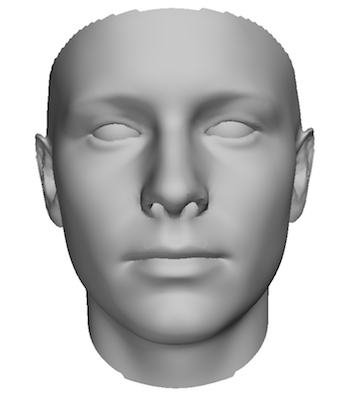
\includegraphics[height=1.9in]{background/images/basel}
		\caption{Basel~\cite{paysan20093d}}\label{fig:db_examples_basel}
	\end{subfigure}
	\begin{subfigure}[b]{0.3\textwidth}
		\centering
		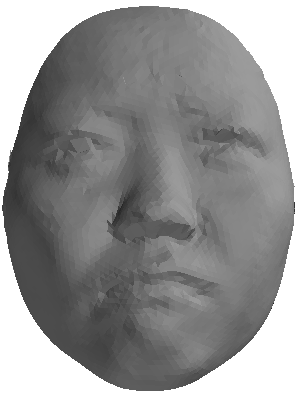
\includegraphics[height=2in]{background/images/bu3d}
		\caption{BU3D-FE~\cite{Yin:2006cc}}\label{fig:db_examples_bu3d}
	\end{subfigure}
	\begin{subfigure}[b]{0.3\textwidth}
		\centering
		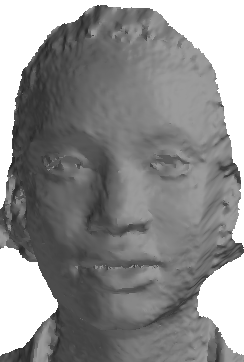
\includegraphics[height=2in]{background/images/bp4d}
		\caption{BP4D-S~\cite{Zhang:2014id}}\label{fig:db_examples_bp4d}
	\end{subfigure} \\
	\begin{subfigure}[b]{0.3\textwidth}
		\centering
		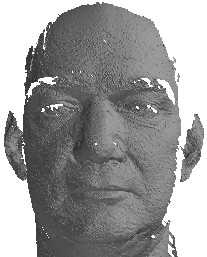
\includegraphics[height=2in]{background/images/frgc}
		\caption{FRGC v2~\cite{phillips2005overview}}\label{fig:db_examples_frgc}
	\end{subfigure}
	\begin{subfigure}[b]{0.3\textwidth}
		\centering
		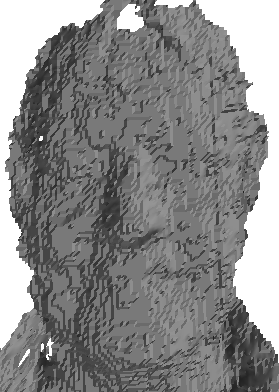
\includegraphics[height=2in]{background/images/biwi}
		\caption{BIWI~\cite{fanelli2013random}}\label{fig:db_examples_biwi}
	\end{subfigure}
	\begin{subfigure}[b]{0.3\textwidth}
		\centering
		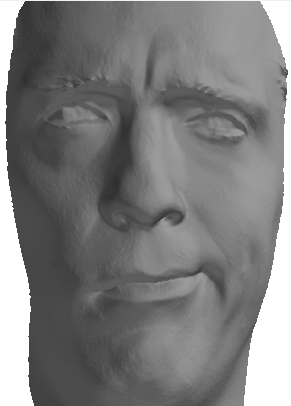
\includegraphics[height=1.9in]{background/images/ict}
		\caption{ICT-3DRFE~\cite{stratou2012exploring}}\label{fig:db_examples_ict}
	\end{subfigure}
	\caption{Examples of the quality of the facial meshes provided in various
	         databases. The meshes were captured by the following systems:
	         \lsubref{fig:db_examples_basel} is from the Basel 3DMM, 
	         which was manually cleaned and captured using a structured light
	         scanner, \lsubref{fig:db_examples_bu3d} by the 
	         3dMD~\cite{3dmd} active stereo system, 
	         \lsubref{fig:db_examples_bp4d} by the 
	         Di4D~\cite{di4d} 4D passive stereo system, 
	         \lsubref{fig:db_examples_frgc} by the 
	         Minolta~\cite{minolta} laser scanning system, 
	         \lsubref{fig:db_examples_biwi} by the 
	         Microsoft Kinect~\cite{zhang2012microsoft} and 
	         \lsubref{fig:db_examples_ict} by a passive stereo 
	         light stage~\cite{debevec2000acquiring}.}
\label{fig:db_examples}
\end{figure}
%%%%%%%%%%%%%%%%%%%%%%%%%%%%%%%%%%%%%%%%
The majority of the databases discussed previously were collected using
commercial apparatus and the focus of the database was the gathering of the
subjects rather than the capturing methodology itself. However, the capturing of
high quality facial surface information is an active area of research and is of
particular interest to the computer graphics community. High quality facial
surface information including mesoscopic details such as fine wrinkles and pores
are necessary for photo-realistic rendering of faces. Photo-realistic rendering
is widely applicable and has seen applications in
films~\cite{borshukov2005universal}, video games~\cite{vonderPahlen:2014kg},
virtual makeup systems~\cite{scherbaum2011computer} and
animatronics~\cite{jung2011believable}. The recovery of these mesoscopic details
requires careful modelling of the interaction between human skin and light. To
this end, many works focus solely on these reflectance characteristics and seek
to provide highly realistic parametric reflectance functions for skin. In this
review, we are only interested in methods that recover realistic 3D shape and
thus do not consider works that focus solely on reflectance function modelling.
For more information about these methods the interested reader should consult
the recent survey on facial appearance capture by \citet{Klehm:2015jb}.

Given the intended use cases for the captured data, facial capturing has focused
on scenarios where both the illumination and camera parameters are tightly
controlled. For this reason, much of the literature focuses on two primary
areas: structured light and stereo. Passive stereo is a photogrammetric method
that requires 2 or more calibrated cameras who's relative positions are used to
infer the 3D position of an objects surface. A key requirement of passive stereo
is a set of correspondences that are shared across multiple camera views. These
correspondences are defined as a set of 2D coordinates that mark salient areas
of the object, visible across multiple cameras. These 2D points are assumed to
represent the 2D projection of a real 3D point onto each camera plane. It is
these correspondences that are used to form geometric constraints for recovery
of 3D positions. However, the computation of these correspondences is itself 
ill-defined as variation in illumination and orientation may cause
the appearance of a true correspondence to vary heavily. Active stereo is
an extension of passive stereo that attempts to simplify the correspondence 
problem by projecting a pattern onto the object at capture time. The pattern
thus provides less ambiguous texture cues for computing correspondences.
In contrast, structured light only requires a single camera and unlike
active stereo this camera must be calibrated with respect to the position of the 
projector supplying the light pattern. The light patterns projected 
by the projector encode the correspondences and 3D information is recovered 
via triangulation.

\textbf{Passive (computational) stereo} is an extremely common technique for
surface recovery and the geometric relationships between two calibrated cameras
are relatively well
understood~\cite{barnard1982computational,seitz2006comparison}. When passive
stereo is applied to reasonably smooth, convex objects in uncluttered scenes, as
is generally the case when capturing faces, it is largely considered a
technology. Commercial systems such as 3dMD~\cite{3dmd} and Di4D~\cite{di4d} are
employed in many areas of entertainment and have been used to capture many of
the high quality databases in \cref{tbl:timeline_db}. Both of these companies
also provided high frame rate systems that are capable of capturing 3D
information at 60+ fps, albeit temporally consistent meshes still require
further post-processing. For this reason, few works in passive stereo focus
solely on the recovery of macroscopic shape using only stereo. Whilst older
works such as that of \citet{Lengagne:1996ej} required 3D models to perform
inference, such as segmentation, on depth maps, modern depth maps are of much
higher quality. Even relatively recent reviews on the subject of passive stereo
applied to faecs~\cite{Leclercq:2005ee} have become obsolete given the price and
quality of modern digital camera systems. For example, the work of
\citet{Beeler:2010dg} demonstrates that standard passive stereo methods can
recover 3D surfaces that contain many high frequency features such as wrinkles.
The highest quality results presented by \citet{Beeler:2010dg} comes from a 7
camera studio setup where per-pixel correspondences and disparity map refinement
is computed in a coarse-to-fine manner. Further constraints are imposed that are
face specific including a smoothness constraint when computing correspondences
and a second-order anisoptropic surface consistency term that reduces smoothing
across depth discontinuities in the disparity maps. Finally, mesoscopic details
are transferred into the mesh via a photometrically consistent surface
refinement procedure. Although the recovered details are not metrically correct,
they do significantly improve the qualitative accuracy of the recovered surface.
Under the assumption that these mesoscopic variations in intensity are linked to
variations in the geometry of the skin, a high-pass filter is first performed in
order to filter out any details captured by stereo. Then, the result of the
stereo is refined along the surface normal direction and is weighted to ignore
high frequency areas caused by larger features such as hairs.

% Need to heavily edit/rewrite this because I got the classification wrong
Structured light methods were some of the
earliest methods for 3D acquisition~\cite{will1971grid}. These methods became
particularly effective for real-time acquisition~\cite{rusinkiewicz2002real} and
more recently structured light was used in the infrared light spectrum for
the original Microsoft Kinect~\cite{zhang2012microsoft}. Although the quality
of output, as depicted for the BIWI head pose database in 
\cref{fig:db_examples_biwi}, is known to be low in the case of the Microsoft
Kinect, structured light is capable of high recovering high quality macroscopic
shape. For example, the Spacetime stereo method of \citet{Zhang:2005ww} was
effectively applied to faces in~\cite{zhang2004spacetime}. Here, 2 projectors
are used in conjunction with 2 stereo pairs (4 cameras) to perform stereo
on a sequence of images. The use of both structured light and multiple frames
allows for the recovery of high quality facial shape. \citet{zhang2004spacetime}
also propose a global optimisation that helps reduce the ridging artefacts
that are common in structured light geometries. Real time capture of 
high-quality facial shape using structured light has also been 
proposed~\cite{zhang2006high,weise2007fast}. \citet{zhang2006high} proposed
a set of custom hardware the enabled 40 FPS capture and reconstruction. The
reconstruction is computed rapidly via a novel three-step phase shifting
algorithm. \citet{weise2007fast}.
%%%%%%%%%%%%%%%%%%%%%%%%%%%%%%%%%%%%%%%%%%%%%%%%%%%%%%%%%%%%%%%%%%%%%%%%%%%%%%%%
